\section{Tahapan Desain}
\label{sec:tahapan-desain}

\begin{figure}[htbp]
    \centering
    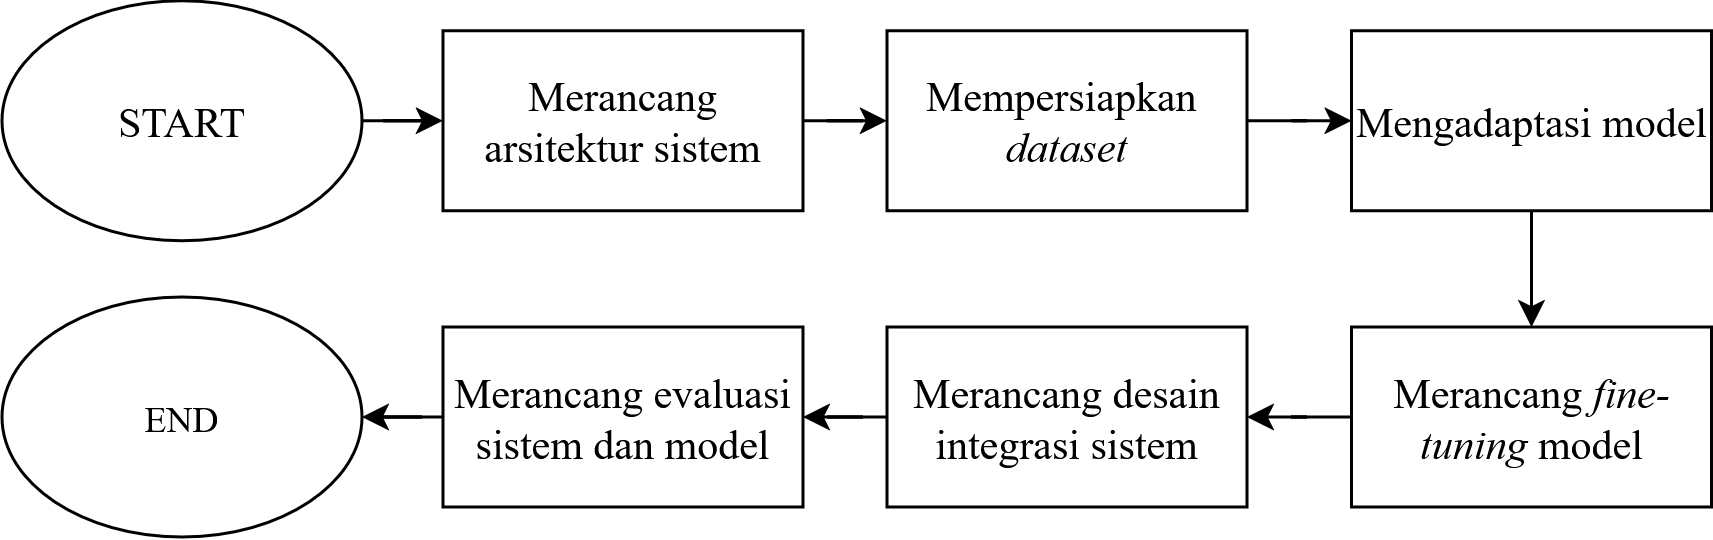
\includegraphics[width=1\textwidth]{images/design-flow.png}
    \caption{Alur kerja tahapan desain sistem pencatatan pengeluaran berbasis \emph{mobile} dengan model \donut}
    \label{fig:design-flow}
\end{figure}

\autoref{fig:design-flow} menunjukkan tahapan desain yang dilakukan untuk mencapai implementasi sistem. Tahapan desain utama mencakup merancang arsitektur sistem, mempersiapkan \dataset, mengadaptasikan model, merancang \emph{fine-tuning} model, merancang desain integrasi sistem, dan merancang evaluasi sistem dan model. Tahapan desain yang dihasilkan akan menjadi dasar untuk mengembangkan sistem pencatatan pengeluaran berbasis \emph{mobile}.

\subsection{Strategi Persiapan Dataset}
\label{subsec:strategi-persiapan-dataset}

Persiapan \dataset{} merupakan tahapan kritis dalam pengembangan sistem ekstraksi data pembayaran. Strategi persiapan \dataset{} dirancang untuk memastikan kualitas dan representativitas data yang akan digunakan untuk melatih model \donut{} yang telah disesuaikan dengan domain pembayaran Indonesia.

\datasetfl{} yang disiapkan mencakup gambar bukti pembayaran dari berbagai jenis aplikasi pembayaran digital dan struk kertas. \datasetfl{} struk kertas yang digunakan untuk melatih model \donut{} adalah \dataset{} CORD-v2\footnote{\href{https://huggingface.co/datasets/naver-clova-ix/cord-v2}{https://huggingface.co/datasets/naver-clova-ix/cord-v2}} (\emph{Consolidated Receipt Dataset for Post-OCR Parsing}). \datasetfl{} ini dibagi menjadi 800 data latih, 100 data validasi, dan 100 data uji. \datasetfl{} ini digunakan untuk melatih model \donut{} agar dapat mengenali dan mengekstrak informasi dari struk pembayaran. \datasetfl{} ini memiliki keterbatasan, yaitu memiliki bagian yang di-\emph{blur}. Keterbatasan ini membuat \donut{} mengalami kesulitan untuk memprediksi struk pembayaran yang penuh.
\begin{figure}[htbp]
    \centering
    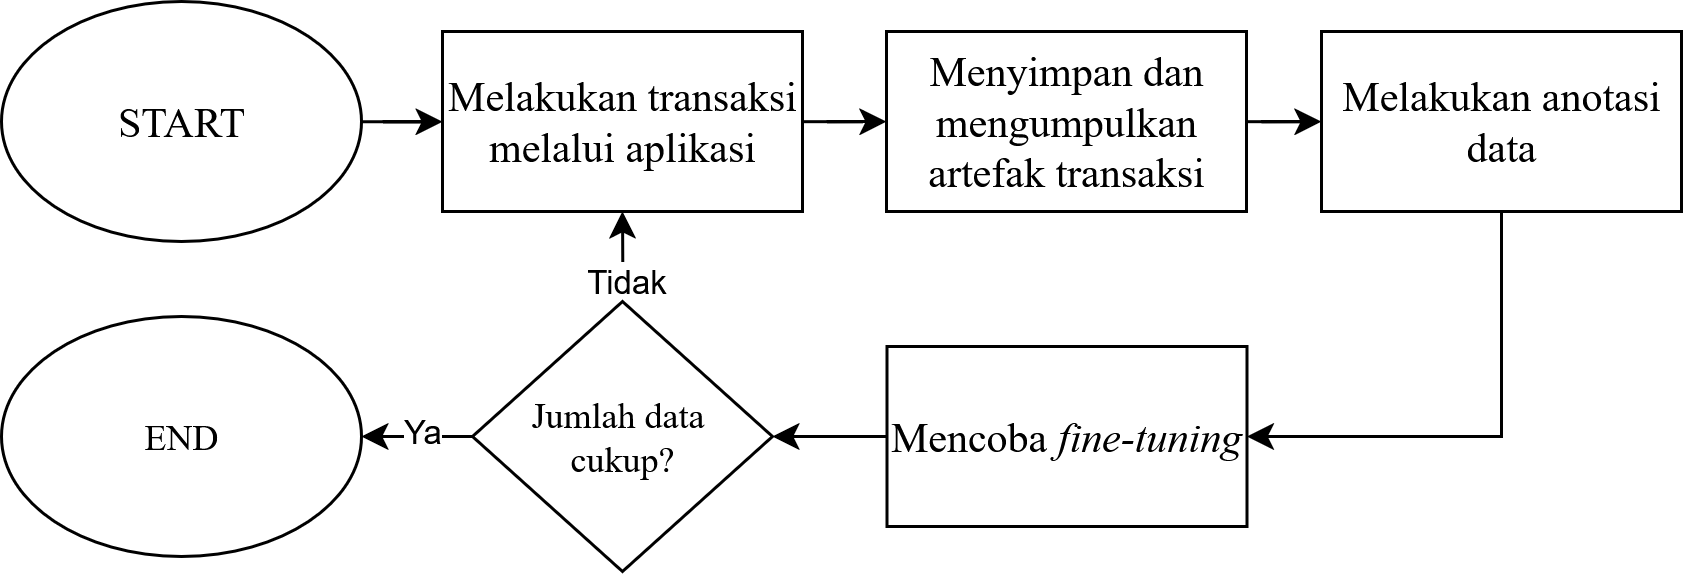
\includegraphics[width=1\textwidth]{images/dataset-preparation-flow.png}
    \caption{Alur kerja persiapan \dataset{} QRIS dan transfer bank}
    \label{fig:dataset-preparation-flow}
\end{figure}

\datasetfl{} yang digunakan untuk melatih model \donut{} adalah \dataset{} QRIS dan transfer yang berisi gambar bukti pembayaran dari berbagai aplikasi pembayaran digital seperti SeaBank, Neobank, BCA, dan \gopay{} yang perlu dipersiapkan secara sistematis. \autoref{fig:dataset-preparation-flow} menunjukkan alur kerja sistematis dalam persiapan \dataset. Proses dimulai dengan melakukan transaksi melalui aplikasi pembayaran dan mengumpukan gambar bukti pembayaran dari berbagai sumber, yaitu aplikasi pembayaran digital (SeaBank, Neobank, BCA, dan \gopay). Total \dataset{} yang dikumpulkan adalah 412 gambar bukti pembayaran QRIS dan transfer dengan format dan jenis dokumen yang bervariasi.

Gambar bukti pembayaran yang telah dikumpulkan kemudian dianotasi secara manual. Proses anotasi dilakukan secara manual untuk menandai informasi penting pada gambar dan memastikan bahwa data yang dianotasikan sesuai. Atribut yang dianotasikan adalah sebagai berikut.
\begin{enumerate}
    \item \iden{}: Kode transaksi yang unik untuk setiap bukti pembayaran.
    \item \total{}: Jumlah pembayaran yang tercantum pada bukti pembayaran.
    \item \ttime{}: Waktu transaksi yang tercatat pada bukti pembayaran.
    \item \target{}: Nama penerima atau tujuan pembayaran.
    \item \app{}: Aplikasi yang digunakan untuk melakukan transaksi.
    \item \type{}: Jenis dokumen berupa QRIS atau transfer.
\end{enumerate}

Proses anotasi ini dilakukan dengan cermat untuk memastikan bahwa setiap informasi yang diperlukan dapat diekstraksi dengan akurat oleh model \donut{}. Hasil anotasi kemudian disimpan dalam format JSON dan kemudian dikonversi menjadi format yang sesuai untuk pelatihan model \donut{}, yaitu format JSONL. 

\datasetfl{} yang telah dianotasi ini kemudian dibagi menjadi tiga \emph{subset}, yaitu data latih, data validasi, dan data uji. Pembagian dilakukan dengan mempertimbangkan distribusi jenis dan variasi jenis dokumen untuk memastikan bahwa setiap \emph{subset} mencakup representasi yang baik dari keseluruhan \dataset. Data latih digunakan untuk \emph{fine-tuning} model, data validasi untuk proses pelatihan, sedangkan data uji digunakan untuk evaluasi akhir kinerja model. 

\emph{Fine-tuning} model kemudian dilakukan untuk memastikan data yang cukup dan tidak mengandung bias yang dapat menyebabkan \emph{overfitting} pada model. Proses pengumpulan data kemudian dihentikan setelah jumlah data dinilai cukup untuk melatih model \donut{} dengan baik.

\subsection{Merancang Arsitektur dan Desain Integrasi Sistem}
\label{subsec:merancang-aristektur-dan-desain-integrasi-sistem}

Subbab ini menjelaskan mengenai struktur dan organisasi sistem yang akan dibangun dari berbagai pandangan arsitektur yang digunakan untuk menggambarkan sistem. Rancangan sistem dibuat dengan mengacu pada kebutuhan fungsional dan nonfungsional yang telah 
dianalisis sebelumnya, untuk memastikan sistem yang dikembangkan memenuhi tujuan dan kebutuhan pengguna.

Pendekatan yang digunakan untuk membuat desain arsitektur ini adalah 4+1 View Model. Model ini mengorganisasikan arsitektur sistem ke dalam lima pandangan yang berbeda, yaitu \emph{scenarios view}, \emph{logical view}, \emph{process view}, \emph{development view}, dan \emph{physical view}. Setiap pandangan memberikan perspektif yang berbeda terhadap sistem sehingga dapat memberikan gambaran yang komprehensif mengenai arsitektur sistem yang akan dibangun. Pendekatan ini memungkinkan proses pengembangan sistem menjadi lebih terstruktur dan sistematis.

\subsubsection{\emph{Scenarios View}}
\label{subsubsec:use-case-view}

\emph{Scenarios View} menunjukkan perilaku sistem dari sudut pandang pengguna melalui pemodelan \emph{use case}. \autoref{fig:bpmn-to-be} menunjukkan \emph{Business Process Model and Notation} (BPMN) untuk \emph{use case} utama sistem, yaitu \emph{share-extract-save}. BPMN ini menunjukkan perbedaan alur kerja dari BPMN sistem saat ini (\emph{As-Is}) yang telah ditunjukkan pada \autoref{sec:analisis-kondisi-saat-ini}. Proses manual yang perlu dilakukan pengguna mulai dari mengekstrak data hingga menyimpan hasil pencatatan pengeluaran ke dalam aplikasi telah diotomatisasi pada sistem yang diusulkan.

\autoref{fig:use-case-diagram} menunjukkan \emph{use case diagram} sistem pencatatan pengeluaran berbasis \emph{mobile}. Diagram ini menggambarkan interaksi antara pengguna dan sistem pada \emph{use case} yang telah diidentifikasikan dari kebutuhan fungsional. \autoref{tab:use-case-list} menyajikan daftar \emph{use case} yang diidentifikasi dalam sistem beserta kode kebutuhan fungsional yang terkait.

\begin{figure}[htbp]
    \centering
    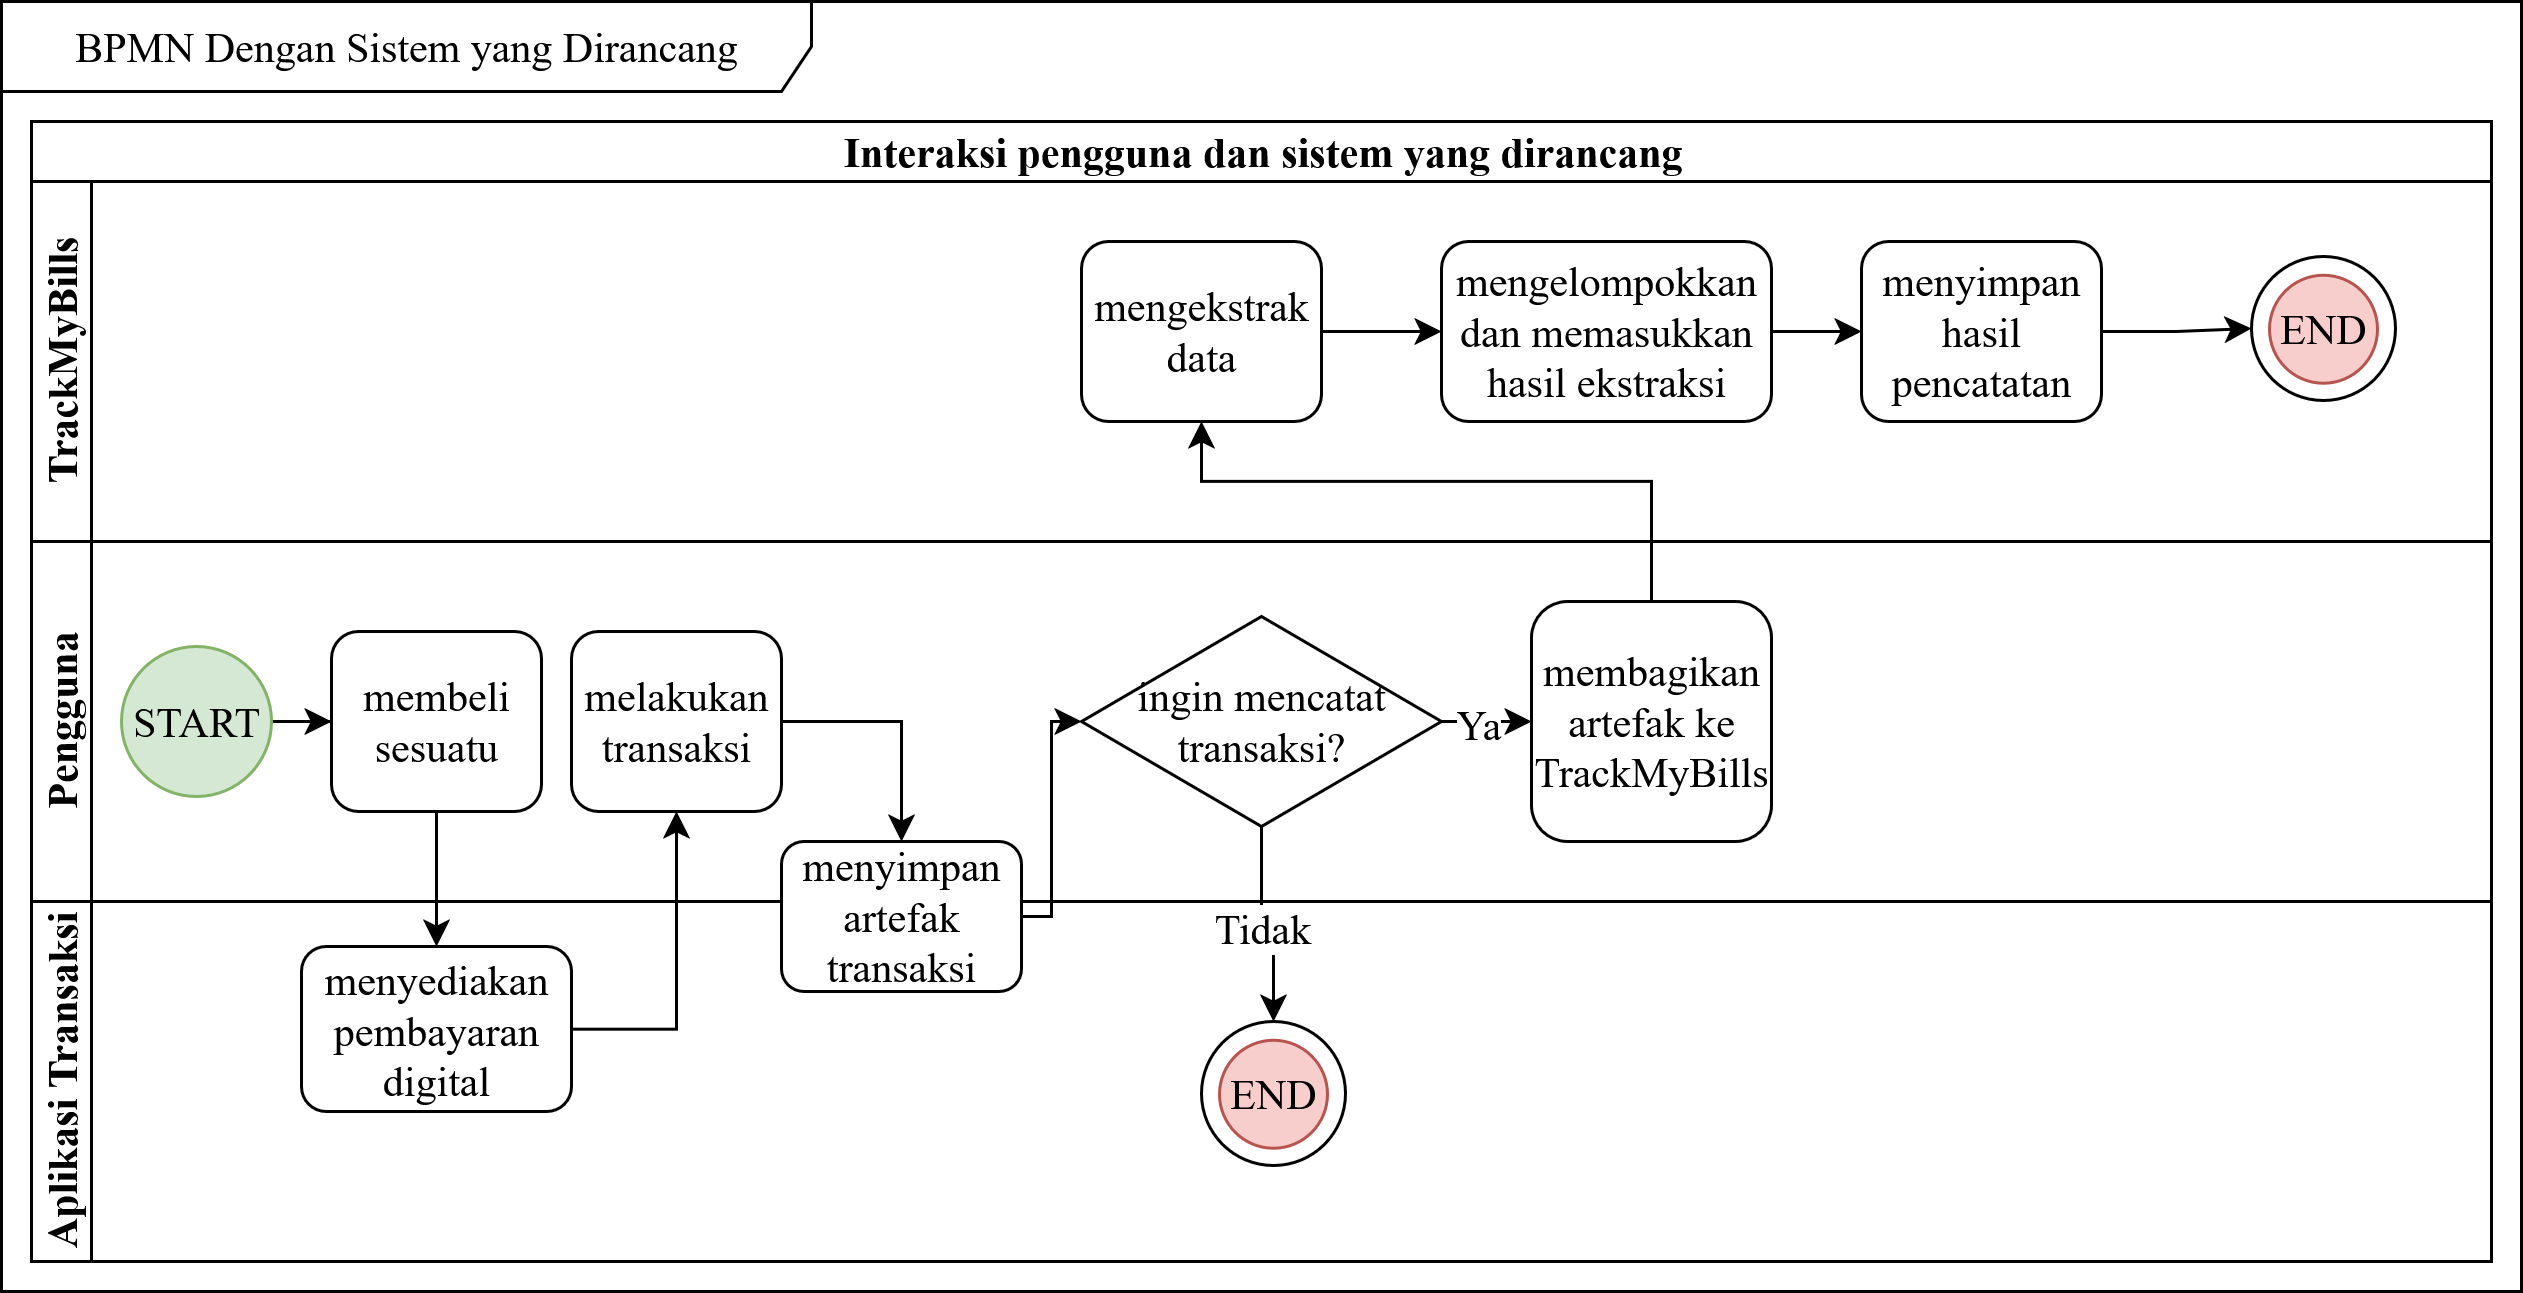
\includegraphics[width=1\textwidth]{images/To-be.png}
    \caption{BPMN untuk \emph{use case} utama sistem (\emph{share-extract-save})}
    \label{fig:bpmn-to-be}
\end{figure}

\begin{figure}[htbp]
    \centering
    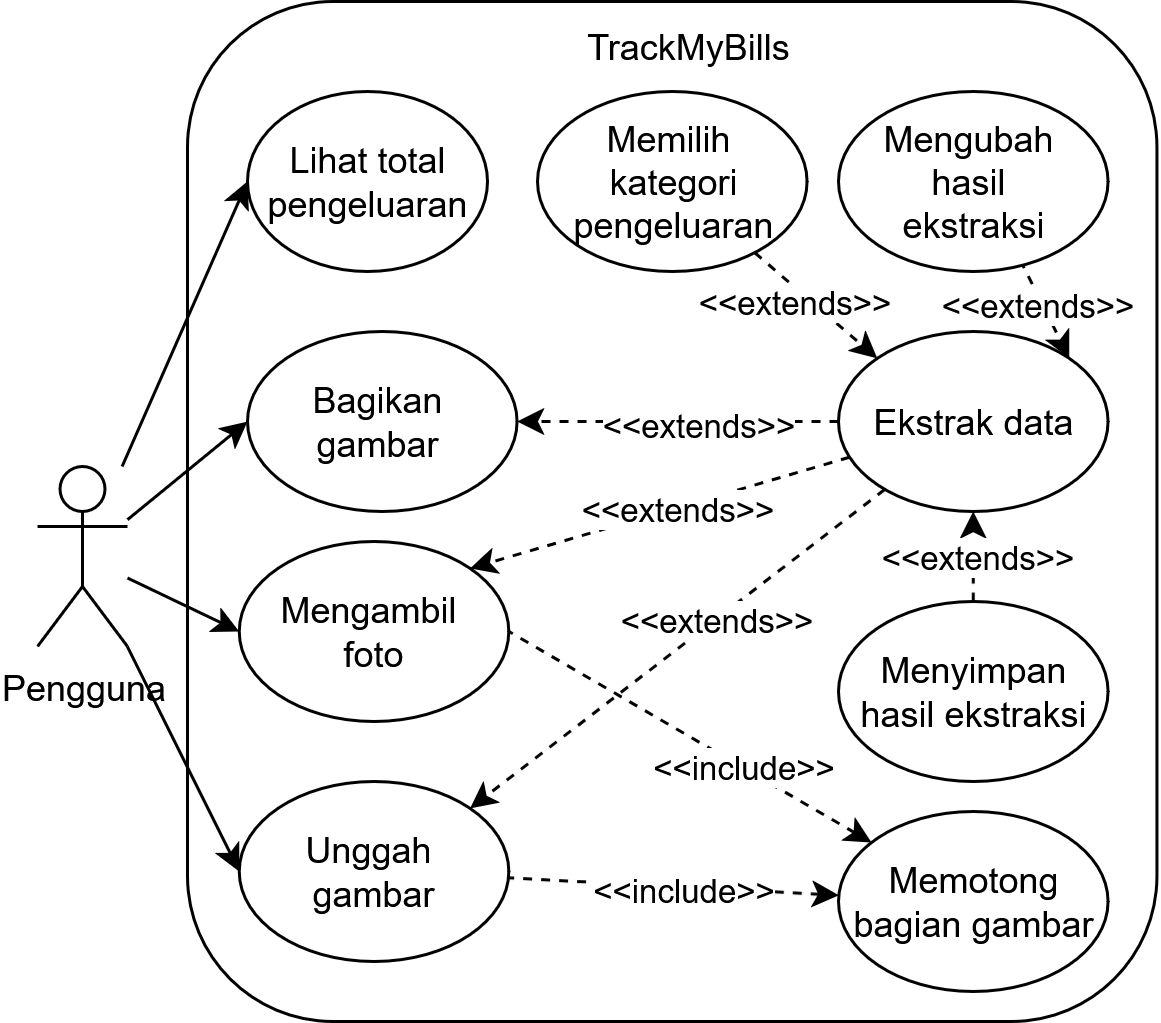
\includegraphics[width=.6\textwidth]{images/use-case-diagram.png}
    \caption{\emph{Use case diagram} sistem pencatatan pengeluaran berbasis \emph{mobile}}
    \label{fig:use-case-diagram}
\end{figure}

\begin{table}[h!]
\centering
\caption{Daftar \emph{use case} sistem pencatatan pengeluaran berbasis \emph{mobile}}
\label{tab:use-case-list}
\begin{tabularx}{\textwidth}{|p{1.6cm}|p{1.5cm}|p{2.8cm}|X|}
\hline
\textbf{Kode \emph{Use Case}} & \textbf{Kode FR} & \textbf{\emph{Use Case}} & \textbf{Deskripsi} \\ \hline
UC-01 & FR-01 & Bagikan gambar & Membagi (\emph{share}) gambar ke sistem \\ \hline
UC-02 & FR-01 & Mengambil foto & Mengakses kamera dari aplikasi dan mengambil foto \\ \hline
UC-03 & FR-01 & Unggah gambar & Memberikan izin mengakses foto dan mengunggah gambar dari galeri \\ \hline
UC-04 & FR-02 & Memotong bagian gambar & Memotong bagian gambar yang diperlukan \\ \hline
UC-05 & FR-03 & Ekstrak data & Mengekstrak data dari gambar yang telah diterima aplikasi \\ \hline
UC-06 & FR-04 & Memilih kategori pengeluaran & Memilih kategori dari data pengeluaran yang diekstrak \\ \hline
UC-07 & FR-04 & Mengubah hasil ekstraksi & Mengubah hasil ekstraksi data sebelum data disimpan \\ \hline
UC-08 & FR-05 & Menyimpan hasil ekstraksi & Menyimpan hasil ekstraksi data dari gambar yang diterima \\ \hline
UC-09 & FR-05 & Lihat total pengeluaran & Melihat total pengeluaran dan pengeluaran per kategori \\ \hline
\end{tabularx}
\end{table}

\subsubsection{\emph{Logical View}}
\label{subsubsec:logical-view}

\begin{figure}[htbp]
    \centering
    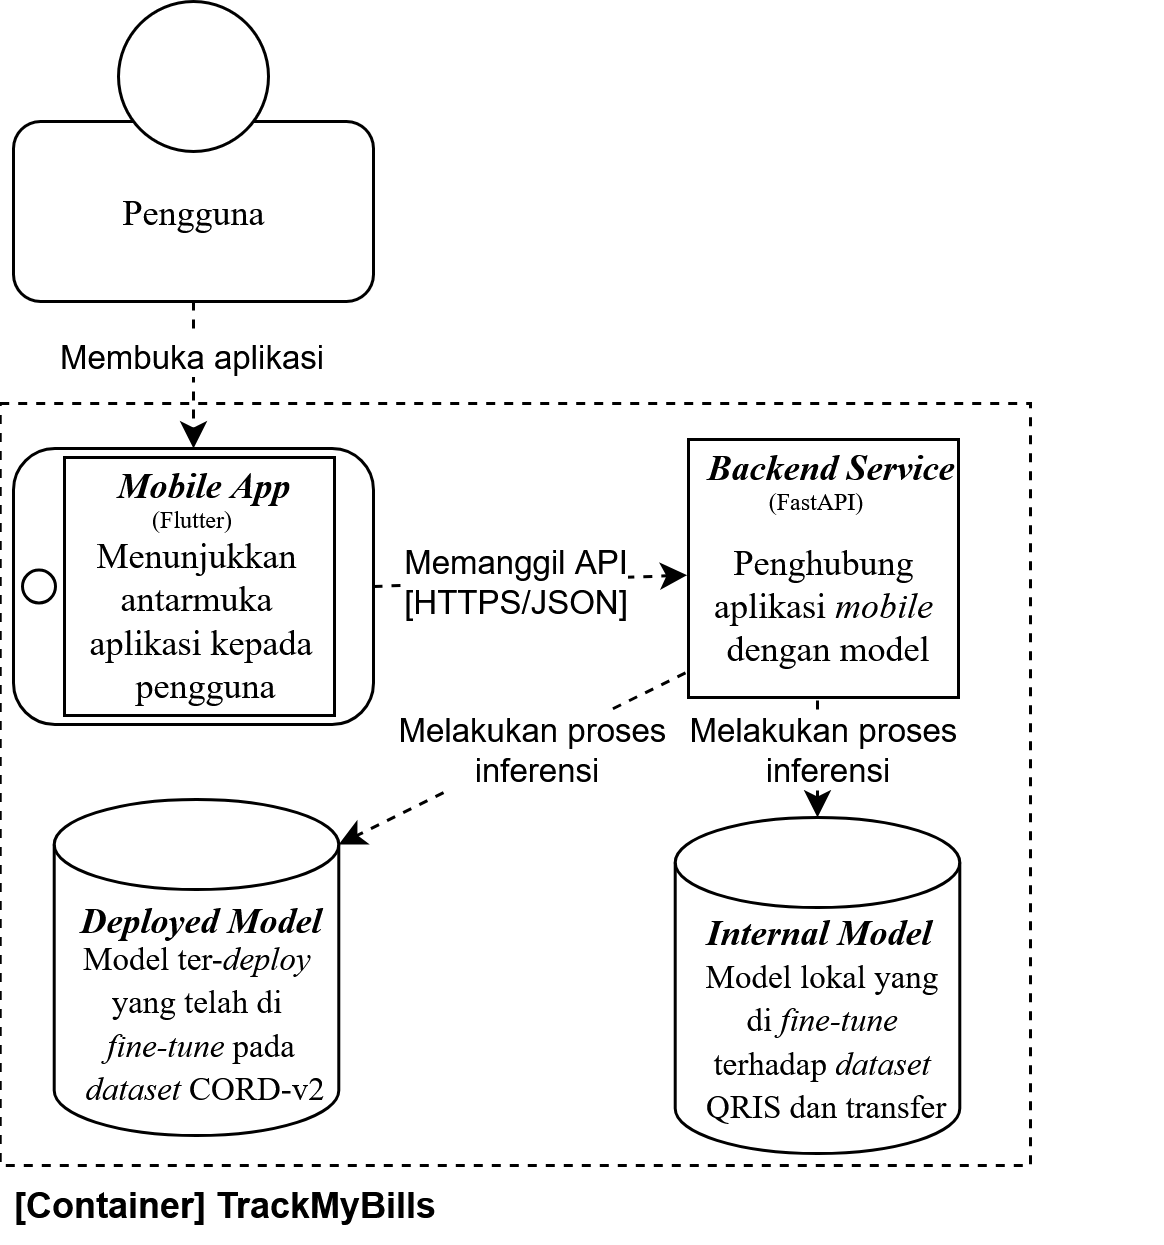
\includegraphics[width=.8\textwidth]{images/container-diagram.png}
    \caption{\emph{Container diagram} sistem pencatatan pengeluaran berbasis \emph{mobile}}
    \label{fig:container-diagram}
\end{figure}

\emph{Logical view} menggambarkan struktur sistem dari sudut pandang logis dari entitas-entitas yang ada dalam sistem secara konseptual. \autoref{fig:container-diagram} menunjukkan \emph{container diagram} sistem pencatatan pengeluaran berbasis \emph{mobile}. Diagram ini menunjukkan bagaimana sistem dibagi menjadi beberapa kontainer, yaitu aplikasi \emph{mobile}, layanan \emph{backend}, model internal, dan model \emph{deployed}. Setiap kontainer memiliki tanggung jawab dan interaksi yang jelas, yang memungkinkan pengembangan dan pemeliharaan sistem menjadi lebih terstruktur.

\autoref{fig:container-diagram} menunjukkan pengguna yang akan berinteraksi dengan aplikasi \emph{mobile}. Aplikasi \emph{mobile} berkomunikasi dengan layanan \emph{backend} melalui API, yang memungkinkan aplikasi untuk mengirim dan menerima data melalui protokol HTTP/JSON. Layanan \emph{backend} bertanggung jawab untuk memproses data dan menghubungkan dengan model internal dan model \emph{deployed}. Model internal dan model \emph{deployed} berfungsi untuk melakukan inferensi dari data yang diterima dari layanan \emph{backend}.




\subsubsection{\emph{Process View}}
\label{subsubsec:process-view}
\emph{Process view} menunjukkan alur kerja sistem dalam menangani proses bisnis dari perspektif interaksi antara pengguna dan sistem. \autoref{fig:activity-diagram} menunjukkan \emph{activity diagram} untuk proses \emph{share-extract-save} yang merupakan proses utama dari sistem yang dibangun. Sebelum proses dimulai, pengguna diasumsikan telah melakukan transaksi dan memiliki artefak transaksi berupa bukti pembayaran QRIS atau transfer. Proses dimulai dengan pengguna memiliki bukti pembayaran dan menggunakan fungsi \emph{share} yang disediakan sistem operasi untuk membagikan artefak tersebut ke aplikasi \emph{mobile}. Aplikasi \emph{mobile} akan menerima artefak tersebut dan menampilkan antarmuka untuk mengonfirmasi artefak yang ingin diproses. Jika artefak sesuai, aplikasi \emph{mobile} akan mengirim bukti pembayaran ke \emph{backend service} untuk divalidasi. Jika validasi berhasil, \emph{backend service} akan memproses bukti pembayaran dengan menggunakan model \donut{} untuk melakukan inferensi. Hasil inferensi akan diproses untuk menjadi format JSON yang sesuai dan dapat diterima aplikasi \emph{mobile}. Aplikasi \emph{mobile} menampilkan hasil pemrosesan untuk dikonfirmasi. Jika hasil telah sesuai dengan keinginan pengguna, pengguna dapat menyimpan hasil tersebut. Jika hasil pemrosesan masih belum sesuai dengan keinginan pengguna, pengguna masih dapat mengubah hasil ekstraksi dan kemudian menyimpan hasil yang telah diperbaiki.

\begin{figure}[htbp]
    \centering
    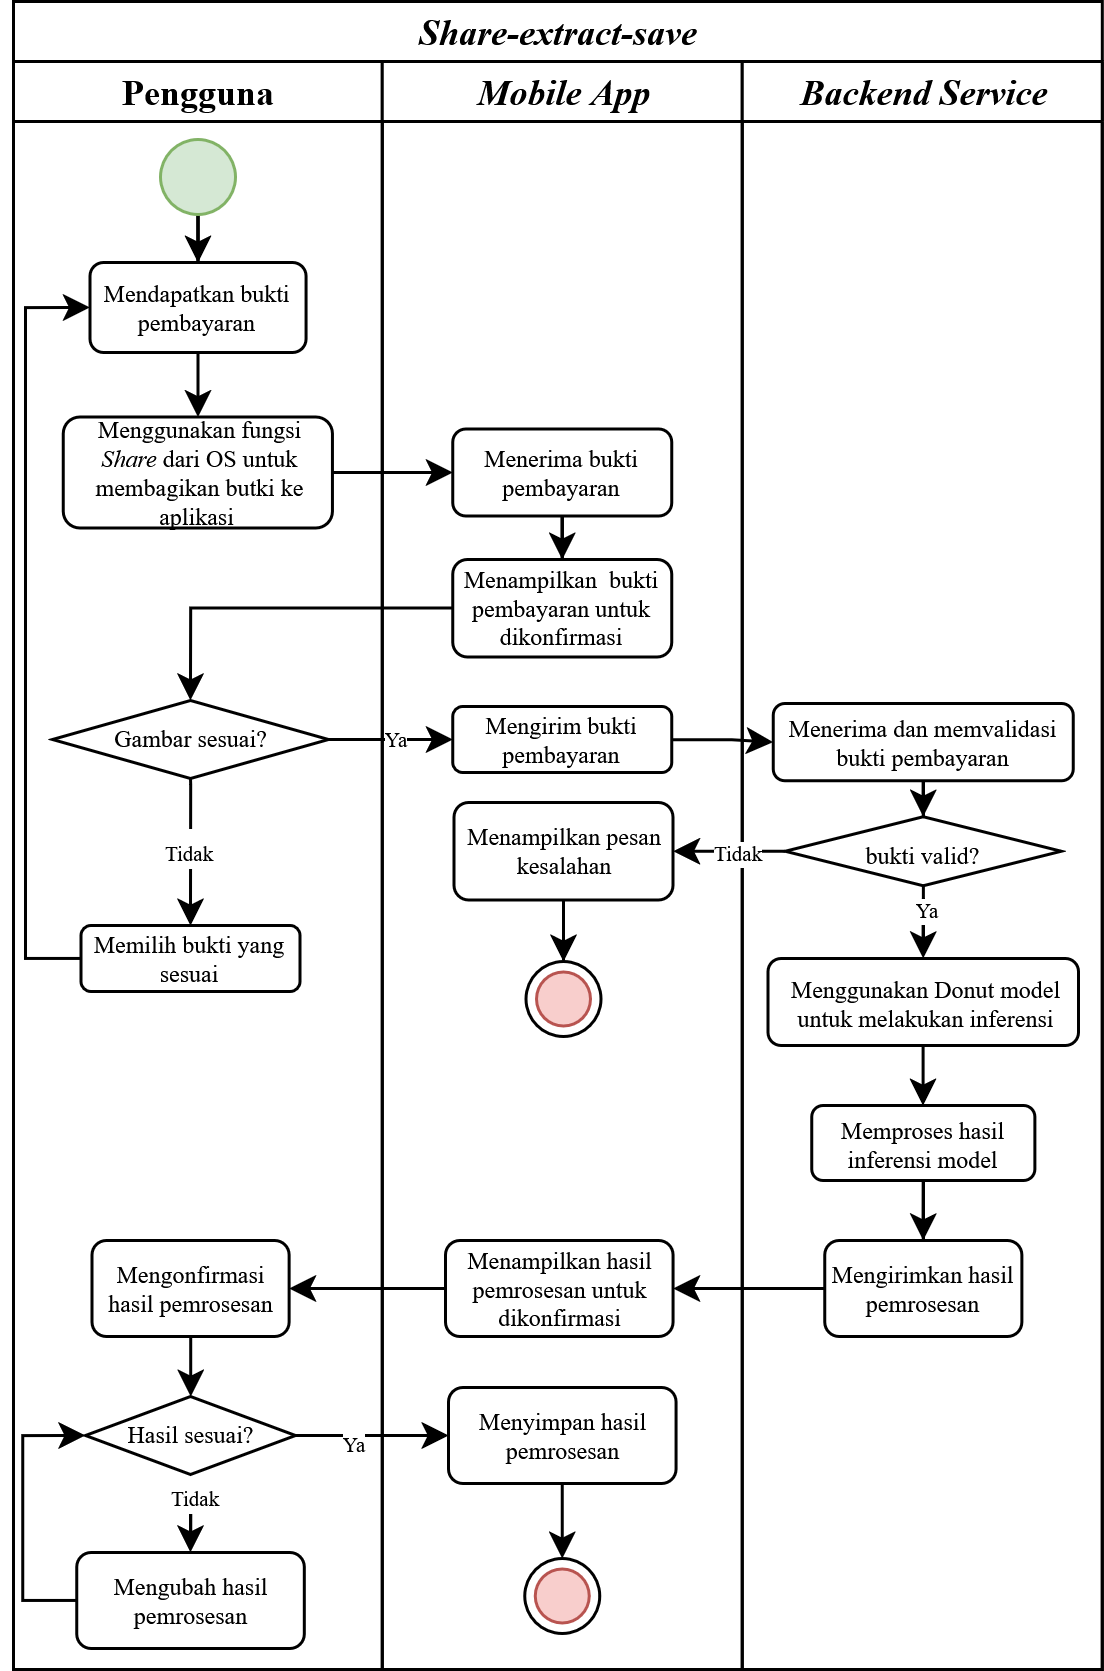
\includegraphics[width=.90625\textwidth]{images/activity-diagram.png}
    \caption{\emph{Activity diagram} untuk proses \emph{share-extract-save}}
    \label{fig:activity-diagram}
\end{figure}


\subsubsection{\emph{Development View}}
\label{subsubsec:development-view}
\emph{Development view} mendefinisikan organisasi sistem dari sudut pandang pengembang. \emph{Development view} membuat pengembang dapat memahami struktur sistem hingga level komponen dan bagaimana komponen tersebut berinteraksi satu sama lain. \autoref{fig:component-diagram} menunjukkan \emph{component diagram} sistem pencatatan pengeluaran berbasis \emph{mobile}. Diagram ini menunjukkan bagaimana sistem dibagi menjadi beberapa komponen, yaitu aplikasi \emph{mobile}, layanan \emph{backend}, model internal, dan model \emph{deployed}. Setiap komponen memiliki tanggung jawab dan interaksi yang jelas dengan kompoenen lainnya untuk memungkinkan pengembangan sistem yang lebih terstruktur.

\begin{figure}[htbp]
    \centering
    % 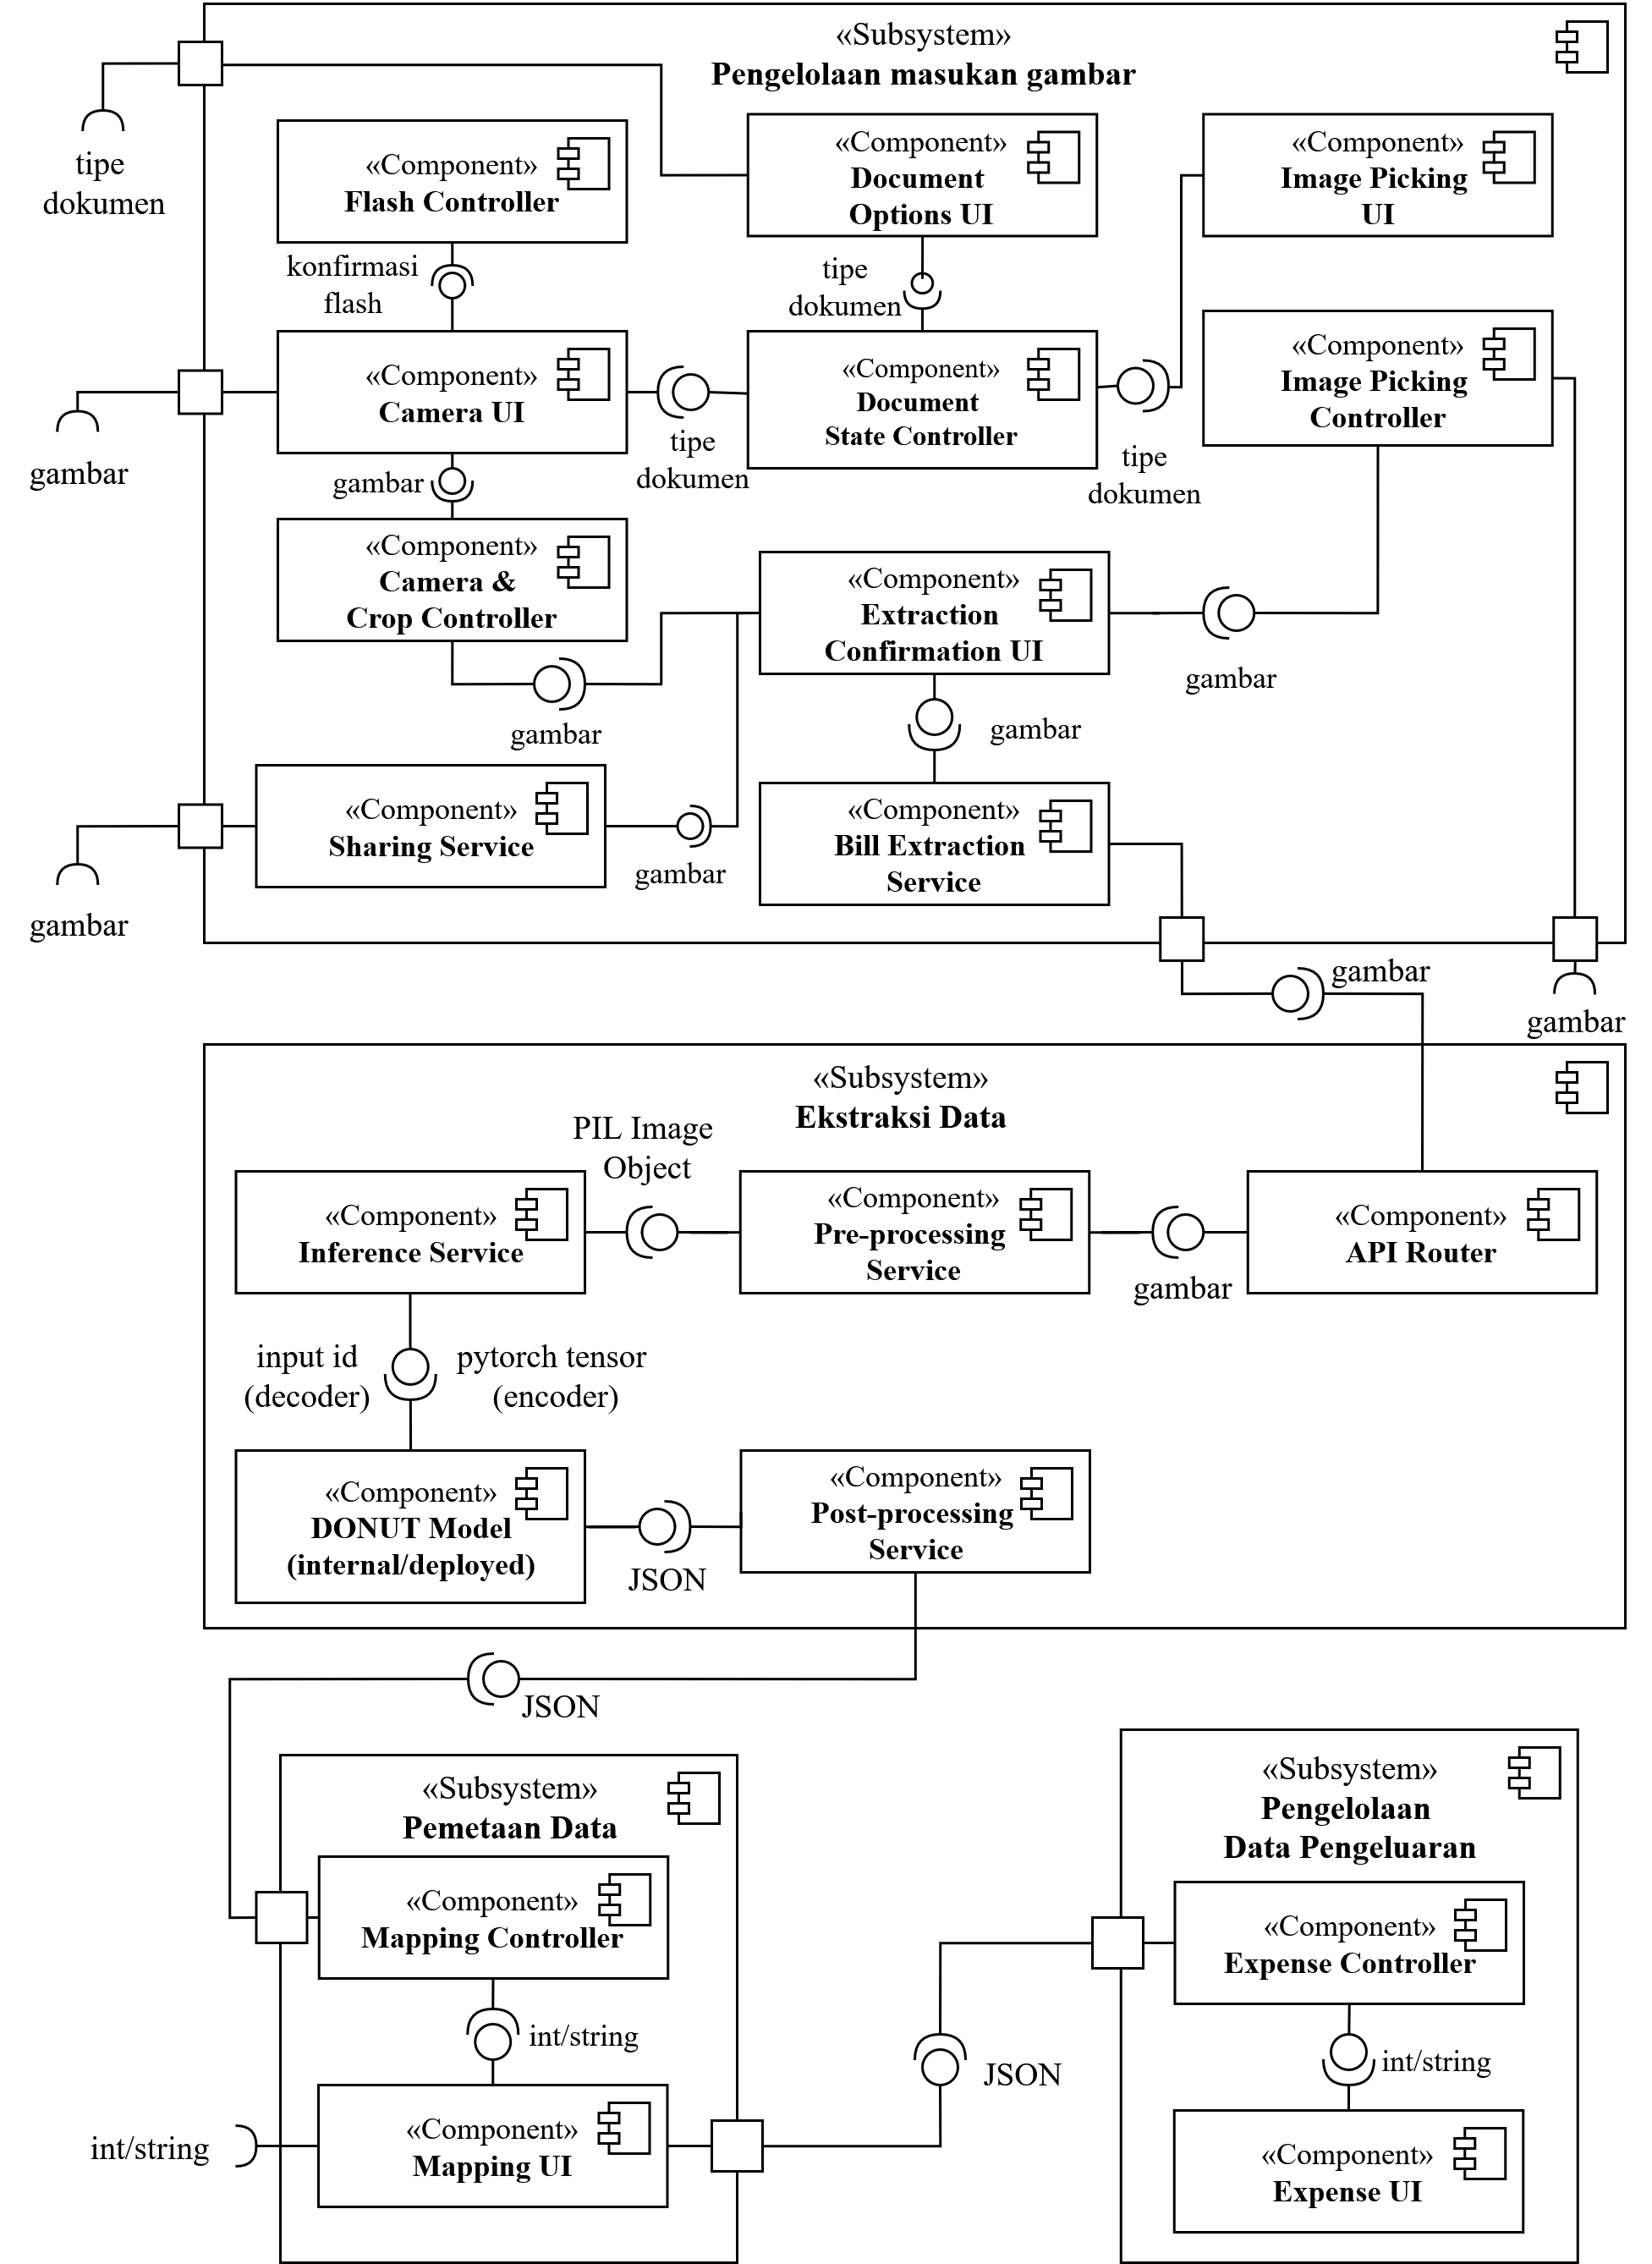
\includegraphics[width=1\textwidth]{images/component-diagram.png}
    \caption{\emph{Component diagram} sistem pencatatan pengeluaran berbasis \emph{mobile}}
    \label{fig:component-diagram}
\end{figure}

\subsubsection{\emph{Physical View}}
\label{subsubsec:physical-view}
\emph{Physical view} menggambarkan bagaimana sistem dipetakan ke infrastruktur fisik, seperti jaringan, server, dan perangkat keras. \emph{Physical view} memastikan bahwa sistem dapat beroperasi dengan baik dalam lingkungan yang telah ditentukan. \autoref{fig:deployment-diagram} menunjukkan \emph{deployment diagram} sistem pencatatan pengeluaran berbasis \emph{mobile} yang menggambarkan aplikasi \emph{mobile}, layanan \emph{backend}, API \emph{Gateway} (ngrok \emph{tunnel}),model internal, dan model \emph{deployed}.
\begin{figure}[htbp]
    \centering
    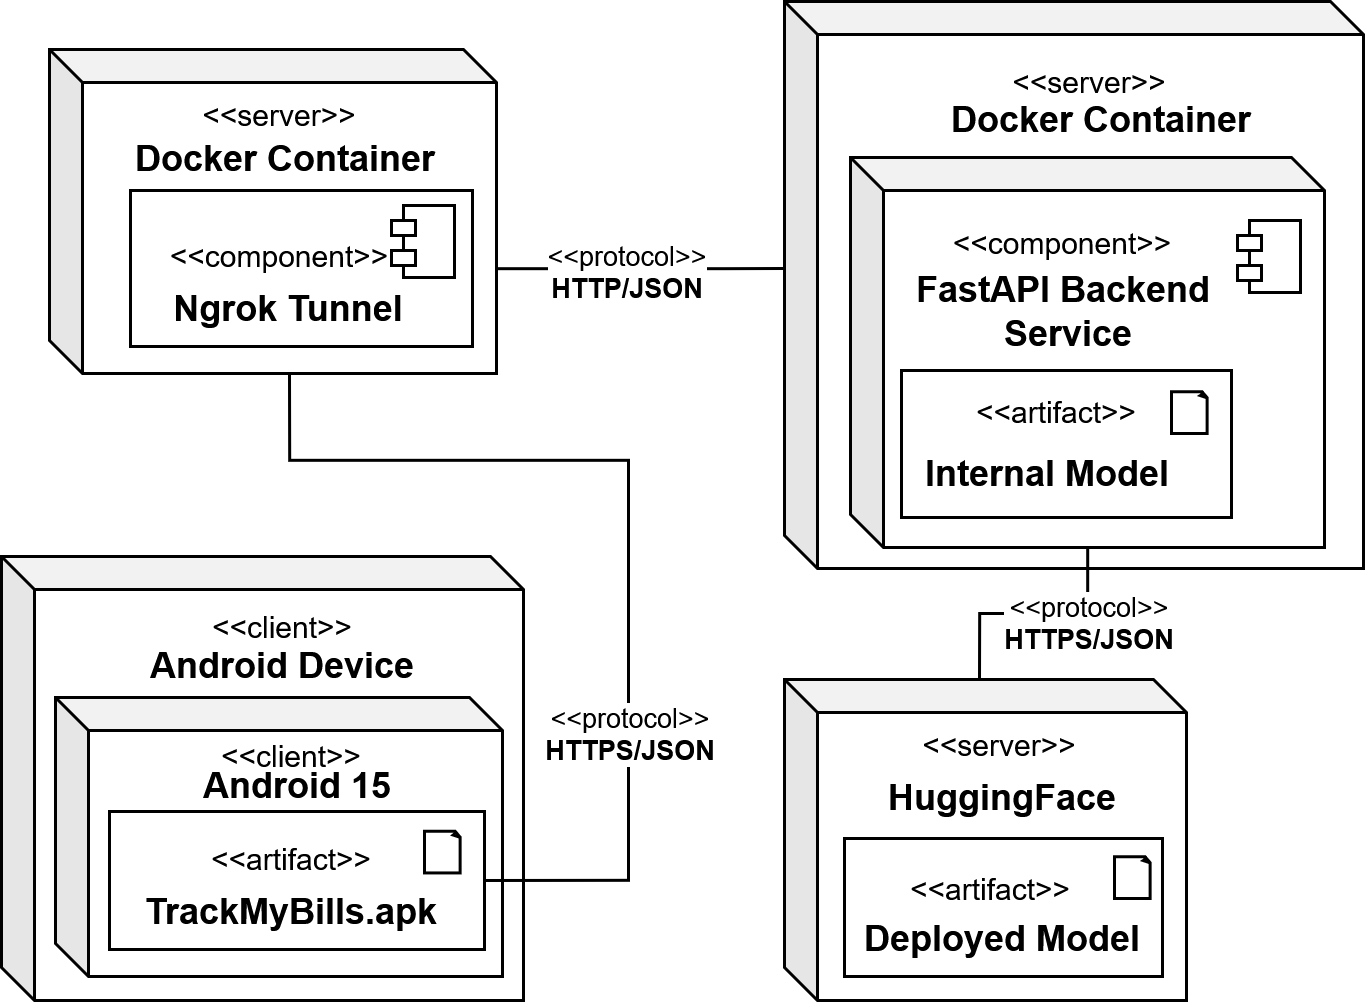
\includegraphics[width=1\textwidth]{images/deployment-diagram.png}
    \caption{\emph{Deployment diagram} sistem pencatatan pengeluaran berbasis \emph{mobile}}
    \label{fig:deployment-diagram}
\end{figure}

\subsection{Perancangan Metodologi Evaluasi}
\label{subsec:perancangan-metodologi-evaluasi}

Perancangan metodologi evaluasi dirancang untuk memberikan penilaian komprehensif terhadap sistem ekstraksi data pembayaran, mencakup aspek teknis dan pengalaman pengguna. Metodologi ini dirancang dengan pendekatan multi-dimensional yang memisahkan evaluasi kinerja model dan evaluasi usabilitas sistem.

% \begin{figure}[htbp]
%     \centering
%     \includegraphics[width=0.8\textwidth]{images/evaluation-framework.png}
%     \caption{Framework evaluasi sistem secara komprehensif}
%     \label{fig:evaluation-framework}
% \end{figure}

\autoref{fig:evaluation-framework} menggambarkan struktur evaluasi yang terbagi menjadi dua cabang utama: evaluasi kinerja model dan evaluasi usabilitas sistem. Pendekatan terpisah ini memungkinkan analisis yang mendalam terhadap aspek teknis dan human-computer interaction secara independen, sambil tetap memberikan gambaran holistik tentang kualitas sistem.

Evaluasi kinerja model dirancang untuk mengukur akurasi ekstraksi data dan klasifikasi dokumen menggunakan metrik standar industri. Metrik yang digunakan mencakup \accuracy{}, \precision{}, \recall{}, F1-\emph{score}, dan \mcer{} dengan ambang batas minimum yang telah ditetapkan berdasarkan standar penelitian terdahulu. \accuracy{}, \precision{}, \recall{}, dan F1-\emph{score} ditetapkan dengan ambang minimum 70\% berdasarkan standar untuk sistem pemahaman dokumen \parencite{kim2021donut, xu2020layoutlm}. \mcer{} ditetapkan dengan ambang maksimum 20\% sebagai indikator akurasi ekstraksi teks yang dapat diterima \parencite{holley2009ocr}.

Implementasi evaluasi model menggunakan pendekatan \emph{unified evaluation} yang dapat menangani kedua jenis model (QRIS-TF dan CORD-v2) dalam satu framework. Sistem evaluasi dirancang dengan fleksibilitas untuk menghitung metrik yang sesuai dengan karakteristik masing-masing model, termasuk evaluasi klasifikasi untuk model QRIS-TF dan fokus ekstraksi untuk model CORD-v2.

Evaluasi usabilitas menggunakan instrumen SUS \emph{score} untuk mengukur pengalaman pengguna Gen Z dalam menggunakan aplikasi mobile. Sampel evaluasi ditetapkan minimum 8 pengguna Gen Z untuk memastikan reliabilitas hasil. Ambang batas SUS ditetapkan pada skor 68 sebagai indikator usabilitas yang dapat diterima, dengan target skor 80+ untuk usabilitas yang excellent \parencite{bangor2009determining}.

Desain protokol evaluasi mencakup skenario penggunaan yang realistis, di mana pengguna diminta untuk memproses berbagai jenis dokumen pembayaran dan memberikan penilaian terhadap kemudahan penggunaan sistem. Evaluasi dilakukan dalam kondisi yang mensimulasikan penggunaan sehari-hari, termasuk variasi kualitas gambar dan jenis dokumen yang beragam.

Metodologi evaluasi juga dirancang untuk mengidentifikasi korelasi antara kinerja teknis dan persepsi pengguna. Analisis ini penting untuk memvalidasi bahwa peningkatan akurasi model berkontribusi terhadap peningkatan kepuasan pengguna. Pendekatan evaluasi yang comprehensive ini memastikan bahwa sistem tidak hanya unggul secara teknis, tetapi juga memberikan nilai praktis bagi pengguna dalam kehidupan sehari-hari.
